\subsection{Write Back stage}

The writeback stage is the final and the most straight-forward 
stage of the pipeline. From the MEM/WB pipeline register the writeback stage
recieves two data words. The WB control signals contains a flag selecting
between the two data words, a write enable signal and a target register
number. After selecting between the two data words all singals are sent
back to the instruction decode stage which contains the register file. The forwarding
unit also takes all the signals as inputs to facilitate forwarding between
write back and instruction decode. Figure~\ref{fig:stage_wb} depicts the architecture of this stage. 

\begin{figure}[h]
        \centering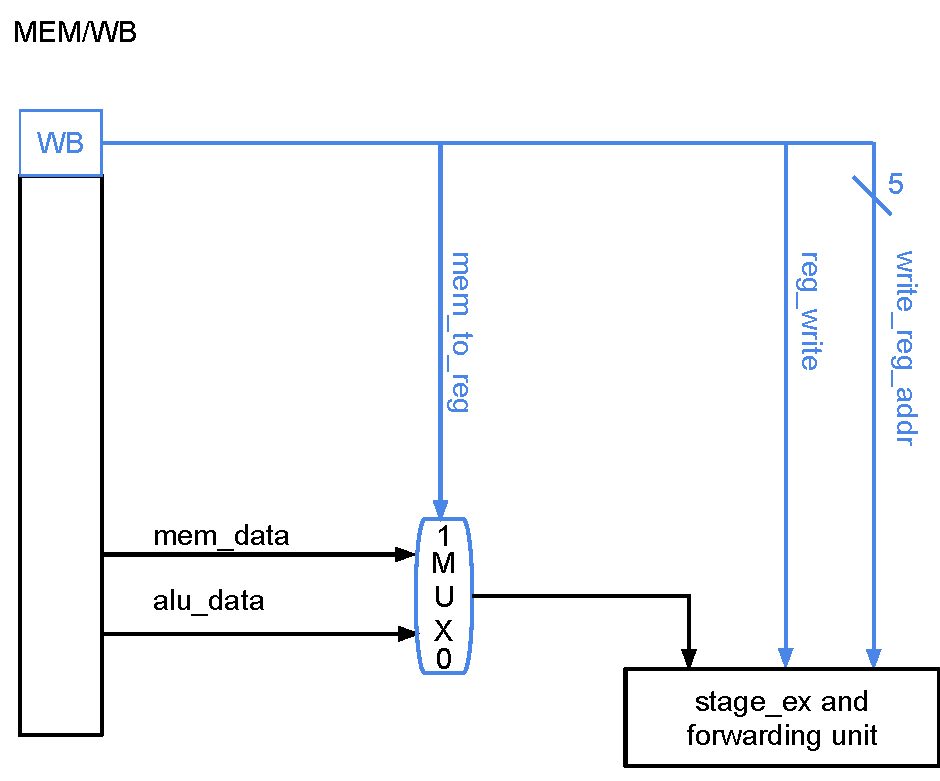
\includegraphics[scale=0.5]{figures/stage_wb}
        \caption{The stage\_wb architecture}
        \label{fig:stage_wb}
\end{figure}